\documentclass[12pt]{article}
\usepackage{listings}
\usepackage[table]{xcolor}
\usepackage{xcolor}
\usepackage{amsmath}
\usepackage{makecell}
\usepackage{graphicx,wrapfig,lipsum}
\usepackage[makeroom]{cancel}
\usepackage{color}   %May be necessary if you want to color links
\usepackage[hidelinks]{hyperref}
\hypersetup{
    colorlinks=false, %set true if you want colored links
    linktoc=all,     %set to all if you want both sections and subsections linked
    linkcolor=blue,  %choose some color if you want links to stand out
}


\graphicspath{ {./images/} }
\newcommand*\xor{\oplus}
\newcommand*\conc{\mathbin\Vert}
\usepackage{array}
\usepackage{amssymb}
\usepackage{biblatex}
\usepackage{placeins}
\usepackage[shortlabels]{enumitem}
\newcommand*\conc{\mathbin\Vert}
\newcommand*\xor{\oplus}
\newcommand{\Mod}[1]{ (\mathrm{mod}\ #1)}
\newcommand{\todo}{\noindent{\color{red} \texttt{\#TODO\#}}}

\addbibresource{references.bib}
\newcolumntype{C}{>$c<$}







\author{Massimo Parisi}
% Make sure you write your name and surname on your solution!
\date{Academic year 2021/2022}	

\begin{document}
%\maketitle

{\center % Center everything on the page
 
%----------------------------------------------------------------------------------------
%	HEADING SECTIONS
%----------------------------------------------------------------------------------------

\textsc{\LARGE Università della Svizzera Italiana}\\[1.5cm] % Name of your university/college
\textsc{\Large Information Security}\\[0.5cm] % Major heading such as course name
\textsc{\large AA 2021/2022}\\[0.5cm] % Minor heading such as course title

%----------------------------------------------------------------------------------------
%	TITLE SECTION
%----------------------------------------------------------------------------------------

\HRule \\[0.4cm]
{ \huge \bfseries InfoSec Summary}\\[0.4cm] % Title of your document
\HRule \\[1.5cm]
 
%----------------------------------------------------------------------------------------
%	AUTHOR SECTION
%----------------------------------------------------------------------------------------

% If you don't want a supervisor, uncomment the two lines below and remove the section above
\Large \emph{Author:}\\
Massimo \textsc{Parisi}\\[1.5cm] % Your name

%----------------------------------------------------------------------------------------
%	LOGO SECTION
%----------------------------------------------------------------------------------------


\includegraphics[scale=0.08]{images/usi-logo.png}\\[2cm] % Include a department/university logo - this will require the graphicx package

%----------------------------------------------------------------------------------------
%	COPYRIGHT SECTION
%----------------------------------------------------------------------------------------


\includegraphics[scale=0.4]{images/copyright.png}\\[1cm]

%----------------------------------------------------------------------------------------
%	DATE SECTION
%----------------------------------------------------------------------------------------

{\large \today}\\[2cm] % Date, change the \today to a set date if you want to be precise
}
%----------------------------------------------------------------------------------------
\newpage


\tableofcontents

\newpage
\section{Basic Crypto}
\subsection{InfoSec objectives}
The main objectives of information security are:
\begin{itemize}
    \item \textbf{Confidentiality}: allow only authorized access to information
    \item \textbf{Integrity}: No unauthorized alteration of data
    \item \textbf{Availability}: information is available to authorized users at all times
    \item \textbf{Authenticity}: 
        \begin{itemize}
            \item \textit{Data origin authentication}: messages originates from claimed source
            \item \textit{Entity authentication}: identification of current source and/or destination
        \end{itemize}
    \item \textbf{Non-repudiation}: prevents an entity from denying previous commitment or actions (e.g. using a digital signature)
\end{itemize}
\subsection{Terminology}
\begin{itemize}
    \item \textbf{Threat}: a potential for violation of security, possible action taken against you
    \item \textbf{Attack}: an assault on system security, a deliberate attempt to exploit one or more vulnerabilities
    \item \textbf{Vulnerability}: specific weakness in (or lack of) security services; a way in which threat can be realized
    \item \textbf{Cryptography}: study of mathematical techniques to enforce security properties
    \item \textbf{Cryptanalysis}: study of how to break cryptographic systems
    \item \textbf{Diffusion}: dissipate plaintext structure into long-range stats in ciphertext (each plaintext bit should affect many ciphertext bits). Its goal is to achieve \textit{Avalanche effect} (switch $1$ bit $\rightarrow$ change at least half ciphertext)
    \item \textbf{Confusion}: Ensure complex ciphertext—key relationship (each key bit should affect many ciphertext bits). Its goal is to achieve \textit{Completeness} (each ciphertext-bit depends on every key-bit)
    \item \textbf{Kerckhoffs‘ Principle}: the security of the encryption scheme must depend only on the secrecy of the key $K_e$, and not on the secrecy of the algorithms.


\end{itemize}
\subsection{Historic Ciphers}
\begin{itemize}
    \item \textbf{Caesar}: a shift cipher in which each character get shifted by a fixed quantity: $c_i=m_i+3 (\bmod 26)\hspace{1em}$ (only 26 possible encryption)
    \item \textbf{Improved Caesar}: remove all non-alphabet characters, use random order of letters (\textit{monoalphabetic} cipher). The key space is much bigger than the previous version ($\approx 2^{88}$) and a simple bruteforce will not work. If we know the language of the message, we can use frequency analysis
    \item \textbf{Playfair}: encode digrams with $5\times 5$ matrix, insert $X$ in between repeating letters. If letters form square, take opposite corners (use letter on same row). If letters are on one row, shift right; if letters are in one column, shift down (wrap around if needed). We can still use frequency analysis to learn some information
    \item \textbf{Vigenère}: different shift for each position, based on a secret keyword. Is it possible to exploit repeating segments of ciphertext (usually digrams/trigrams) and learn the length of the key. If the key length is known, we can try to break multiple monoalphabetic ciphers (using frequency analysis). One possible improvement is \textit{autokeying}, so after the key we continue to encrypt with the plaintext as key. This can still be broken with frequency analysis (English text encrypted with English text)
    \item \textbf{Vernam (OTP)}: it is basically Vigenère with a random key that as the same length of the plaintext. OTP has been mathematically shown to be unbreakable (if you never EVER repeat the key). Nonetheless, it has serious limitation (we should have truly random keys without reuse, really big keys, key distribution problem)
    %\item \textbf{Permutation/Transpostion}: Scytale Staff, Rail Fence Cipher, (Ordered) Route Cipher,Single/Double Transposition, etc.
\end{itemize}


\section{Feistel Ciphers}
An ideal (block) cipher should use ideal keys that can map any plain text block to any cipher block, but these kind of keys would need $2^n\cdot n$ bits, and that is impractical. For this reason we started using the so-called \textbf{Feistel Networks}, used in order to build an \underline{invertible} random permutation $E:P\leftrightarrow C$ using a \underline{non-invertible} random function $f$ as a building block. The basic building block of a Feistel cipher are permutation, substitution and XOR. 
Given a list of round keys $[K_0,...,K_n]$, a Feistel cipher usually perform the following steps:
\begin{itemize}
    \item Split plaintext block $P$ into two equal halves $L_0$ and $R_0$
    \item For each round $i$, it alternately
    \begin{itemize}
        \item Apply non-invertible function $F$ to one half (using $K_i$)
        \item XOR the result onto the other half 
    \end{itemize}
    (e.g. $L_{i+1} = L_i \text{ and } R_{i+1} = R_i \xor F(K_i, L_i)$)
    \item After $n$ rounds, concatenate $L_n$ and $R_n$ to obtain the ciphertext $C$
\end{itemize}
Feistel ciphers presents different advantages, like the fact that encryption and decryption use the same algorithm: in order to decrypt, we use the ciphertext as input and reverse the order of the keys.

\subsection{DES}
\textit{Data Encryption Standard}, or DES, is one of the most famous Feistel cipher. It consists of the following steps:
\begin{enumerate}
    \item Initial permutation (IP)
    \begin{description}
    \item[Note:] unless we are using 3-DES, this step does not help
    \end{description}
    \item 16 Feistel rounds
    \item Swap and Inverse permutation (IP$^{-1}$)
\end{enumerate}
In the Feistel rounds we use the \textit{Mangler} function as $F$, that consist of:
\begin{enumerate}
    \item Expansion ($32\rightarrow 48$ bits)
    \item XOR with $K_i$
    \item \underline{Non-linear} Substitution (with S-boxes)
    \begin{description}
    \item[Note:] S-boxes design is unclear (slight changes can affect security)
    \end{description}
    \item Permutation (with P-boxes)
\end{enumerate}
\subsubsection{Multi-DES}
Simple DES has been cracked (bruteforce), so stronger version of DES has been created:
\begin{itemize}
    \item 2DES: encrypt twice (with 2 different keys)
    \begin{description}
    \item[Note:] it can be subject to a \textit{"Meet in the middle"} attack
    \end{description}
    \item 3DES: encrypt three times (with 2 or 3 different keys)
\end{itemize}

\section{AES}
\textit{Advance Encryption Standard}, or AES, is a non-Feistel cipher.
\subsection{General info}
\begin{itemize}
    \item Block size: 128 bits
    \item Key size: 128/192/256 bits
    \item Rounds: 10/12/14
\end{itemize}
\subsection{Number Theory}
{\color{blue} [skip modular addition, multiplication,etc.]}

\subsection{Galois Fields}
For a given prime $p$, we can define the \textit{finite field of order $p$}, $GF(p)$, as the set $Z_p$ of integers ${0,...,p-1}$ together with the arithmetic operations $\Mod p$.
In order to not waste bit and "fit" directly a finite field into our bytes, we need $GF(2^n)$, but they works differently when using operations.
\subsubsection{Polynomial Arithmetic}

$GF(p^n)$ means that 
\begin{itemize}
    \item we want coefficients in $GF(p)$ ($p=2\rightarrow$ coefficients can only be 0 or 1)
    \item the result of each operations as to be reduced using $\Mod{m(x)}$ where $m(x)$ is some irreducible polynomial with order $n$
\end{itemize}
\begin{center}
    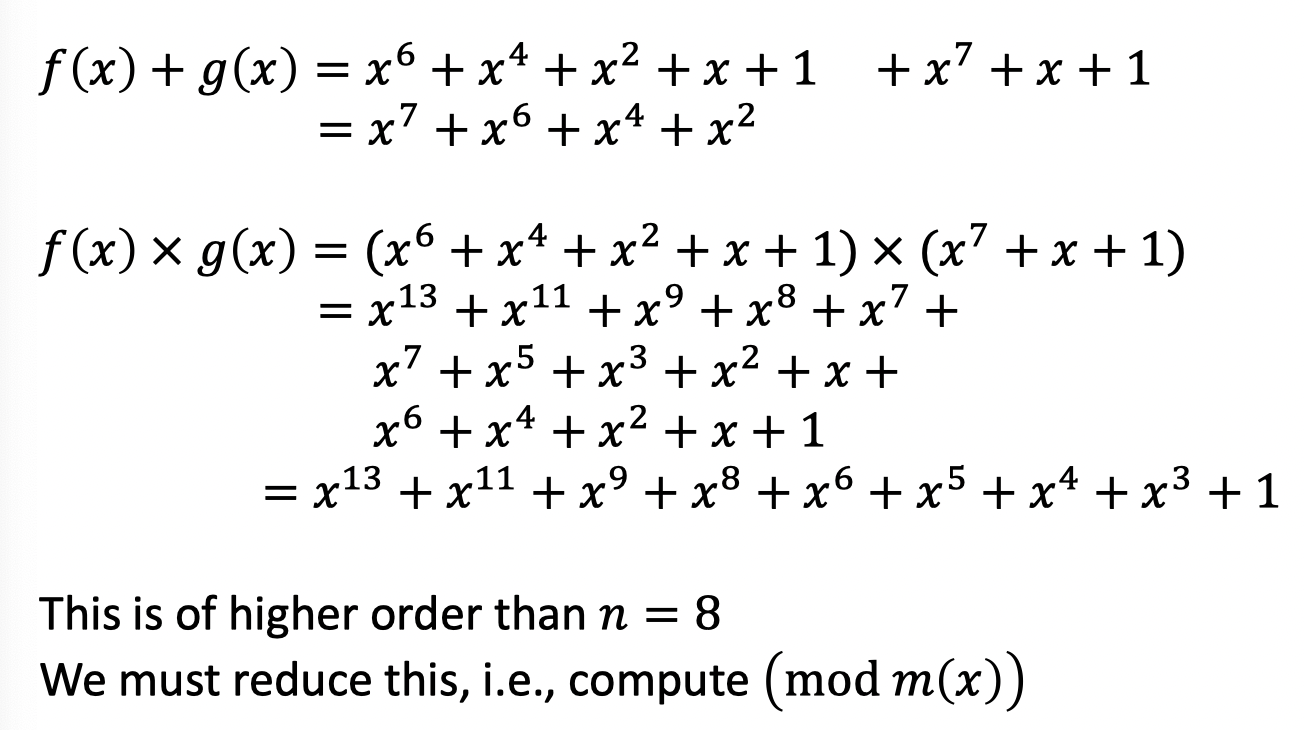
\includegraphics[scale=0.2]{images/gf1.png}
    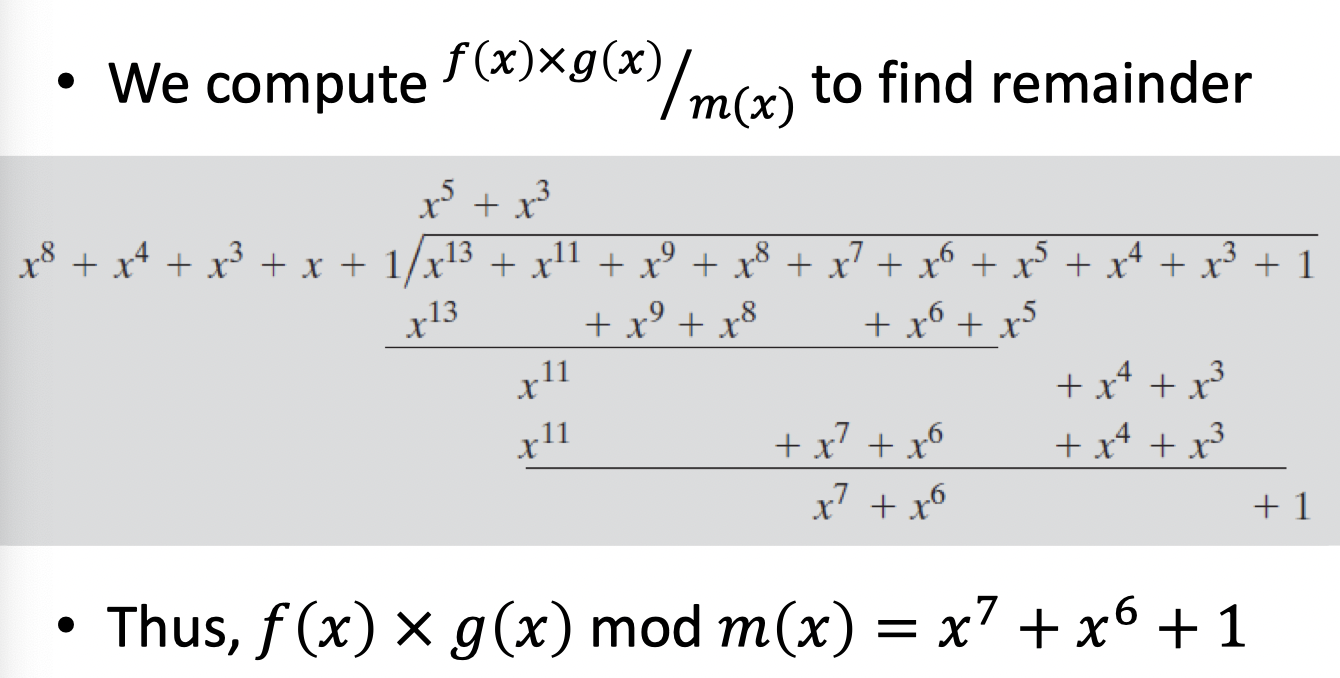
\includegraphics[scale=0.2]{images/gf2.png}
\end{center}

\subsection{AES Structure}
\begin{enumerate}
    \item \textbf{Substitute bytes}: uses an S-box to perform a $b$ byte substitution of the block
    \item \textbf{ShiftRows}: A simple permutation
    \item \textbf{MixColumns}: A substitution that makes use of arithmetic over GF($2^8$)
    \item \textbf{AddRoundKey}: A simple bitwise XOR of the current block with a portion of the expanded key
\end{enumerate}
AES begins with AddRoundKey, followed by $9$ rounds (128-bit) with all $4$ stages and final round with only $3$ stages (skip MixColumns). In order to have the right length for the key, we also perform a \textbf{key expansion}.
\section{Block Modes}
\subsection{Electronic Codebook - ECB}
\begin{wrapfigure}{r}{0.3\textwidth}
\vspace{-20pt}
\fbox{
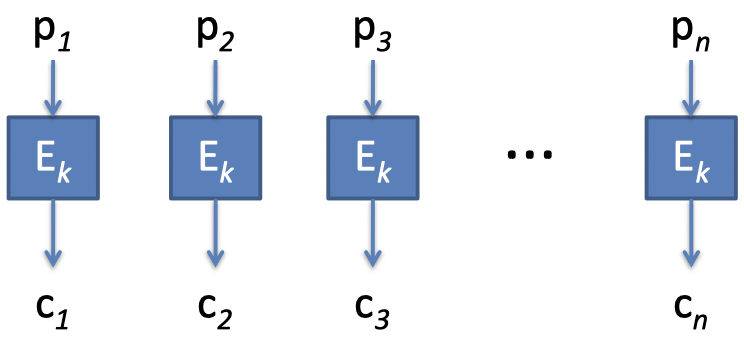
\includegraphics[scale=0.5]{images/ecb.png}}
\end{wrapfigure}
Simplest block mode, just cut the message into $m-$bit blocks and apply the cipher function to each block. 
The problem is that if we repeat a plaintext block, we obtain the same cipher blocks. A first way to improve ECB would be to XOR each plaintext block with random number, but still we will have problems: now we have twice as much data to transmit and message modification is easy.

\subsection{Cipher Block Chaining - CBC}
\begin{wrapfigure}{r}{0.3\textwidth}
\vspace{-50pt}
\fbox{
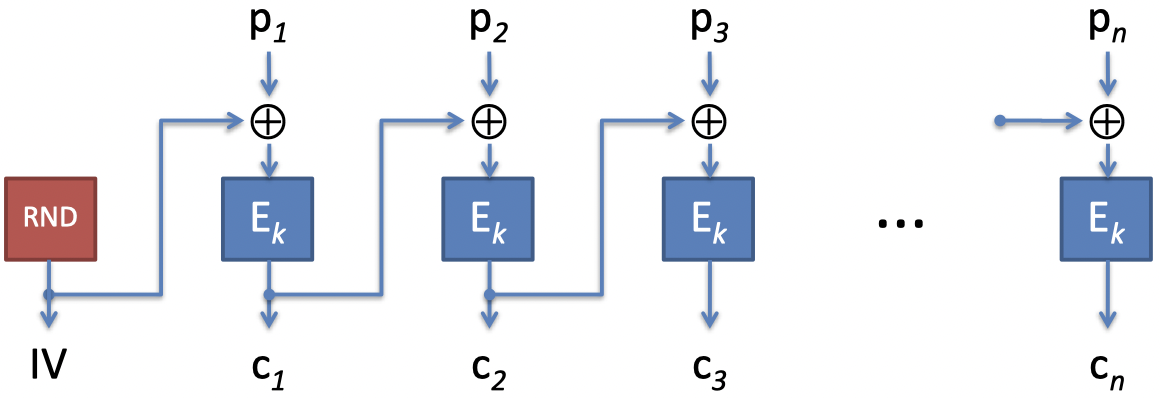
\includegraphics[scale=0.35]{images/cbc.png}}
\end{wrapfigure}
Each block of plaintext is XORed with the preceeding block of ciphertext before encryption. It uses a random \textit{initialisation vector} $IV$ that should never be reused and should stay secret.


\subsection{Cipher Feedback - CFB}
\begin{wrapfigure}{r}{0.3\textwidth}
\vspace{-60pt}
\fbox{
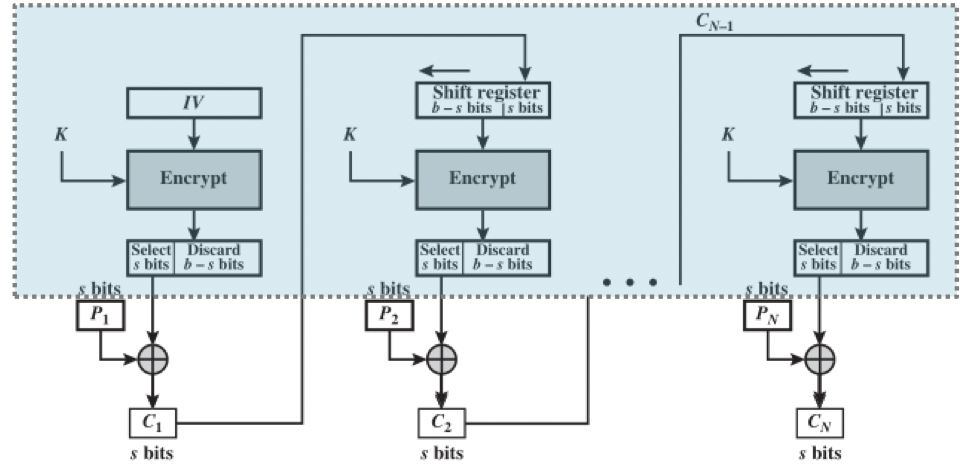
\includegraphics[scale=0.4]{images/cfb.png}}
\end{wrapfigure}
Preceeding ciphertext is used as input to encryption algorithm, to produce pseudorandom output that is XORed with plaintext. Can work on subset of $j$ bits instead of entire blocks.


\subsection{Counter Mode - CTR}
\begin{wrapfigure}{r}{0.3\textwidth}
\vspace{-50pt}
\fbox{
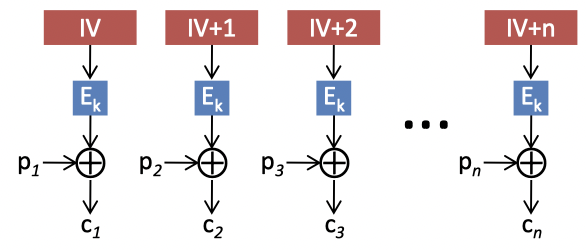
\includegraphics[scale=0.55]{images/ctr.png}}
\end{wrapfigure}
Each plaintext block is XORed to encrypted counter. Counter gets incremented for each subsequent block.


\begin{wrapfigure}{r}{0.3\textwidth}
\vspace{-50pt}
\fbox{
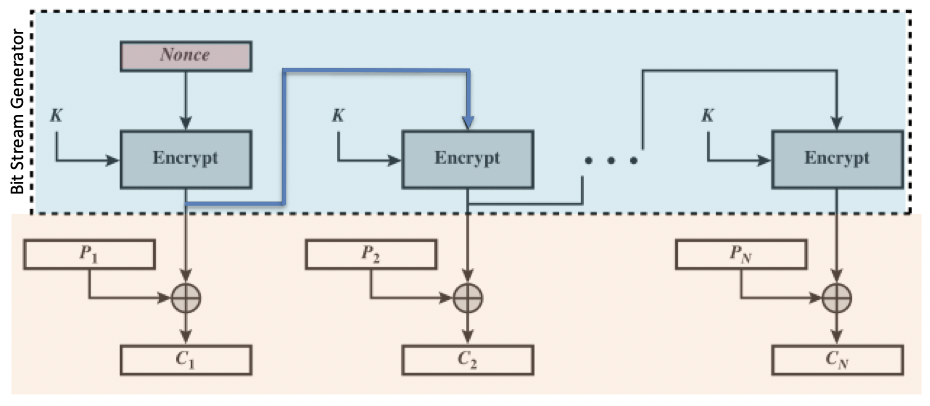
\includegraphics[scale=0.4]{images/ofb.png}}
\end{wrapfigure}
\subsection{Output Feedback - OFB}
Similar to CFB, except that instead of ciphertext, it uses preceeding output of encryption function as input to the successive encryption function.

\section{Stream Ciphers}
A \textbf{stream cipher} operates on one plaintext symbol at a time and use generator function to create pseudo-random keystream. Ideally, we should use a \textit{true random number generator} (TRNG), but they are usually slow, for this reason we use \textit{pseudo-random number generator} (PRNG). A PRNG should have \textit{forward and backward unpredictability}. Let's see some famous PRNGs.
\subsection{Linear Congruential Generator}
The random number sequence $\{X_n\}$ is obtained as $X_{n+1} = (a\cdot X_n + c) \Mod{m}$
It goes without saying that in this case the selection of values for $(a,c,m)$ is critical in developing a good PRNG.
\subsection{Blum Blum Shub (BBS) Generator}
One of the most commonly used PRNGs. The random number sequence $\{X_n\}$ is obtained as follow
\begin{enumerate}
    \item Choose two prime $(p,q)$ s.t. $p\equiv q\equiv 3 \Mod{4}$
    \item Let $n=p\times q$
    \item Choose random $s$ such that $\texttt{gcd}(s,n)=1$
    \item Start from $X_0=s^2 \Mod{n}$
    \item If we want $n$ bits, we repeat $n$ times the following
    \begin{enumerate}
        \item Compute $X_i=(X_{i-1})^2 \Mod{n}$
        \item Take only the LSB from $X_i$
    \end{enumerate}
\end{enumerate}

\subsection{PRNGs using block modes}
\begin{wrapfigure}{r}{0.3\textwidth}
\vspace{-65pt}
\fbox{
\begin{center}
    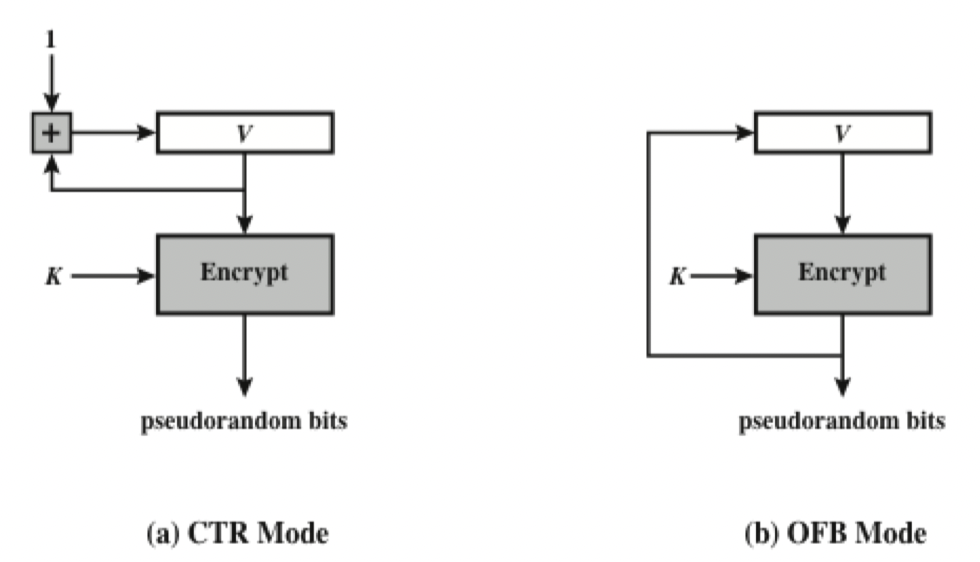
\includegraphics[scale=0.3]{images/prng.png}
\end{center}}
\end{wrapfigure}
It is also possible to create a PRNG starting from a CTR or an OFB mode: they just need a key $K$ and an initial vector $V_0$ (that can be fix, e.g. $V_0=0$)

\subsection{RC4}
RC4 is a variable key size stream cipher. To generate the key stream, the cipher makes use of a secret internal state which consists of two parts:
\begin{itemize}
    \item A permutation of all 256 possible bytes ($S$)
    \item Two 8-bit index-pointers ($i$ and $j$).
\end{itemize}
The permutation is initialized with a variable length key using the key-scheduling algorithm (KSA). Then the stream of bits is generated by a pseudo-random generation algorithm.
\begin{center}
    \fbox{
    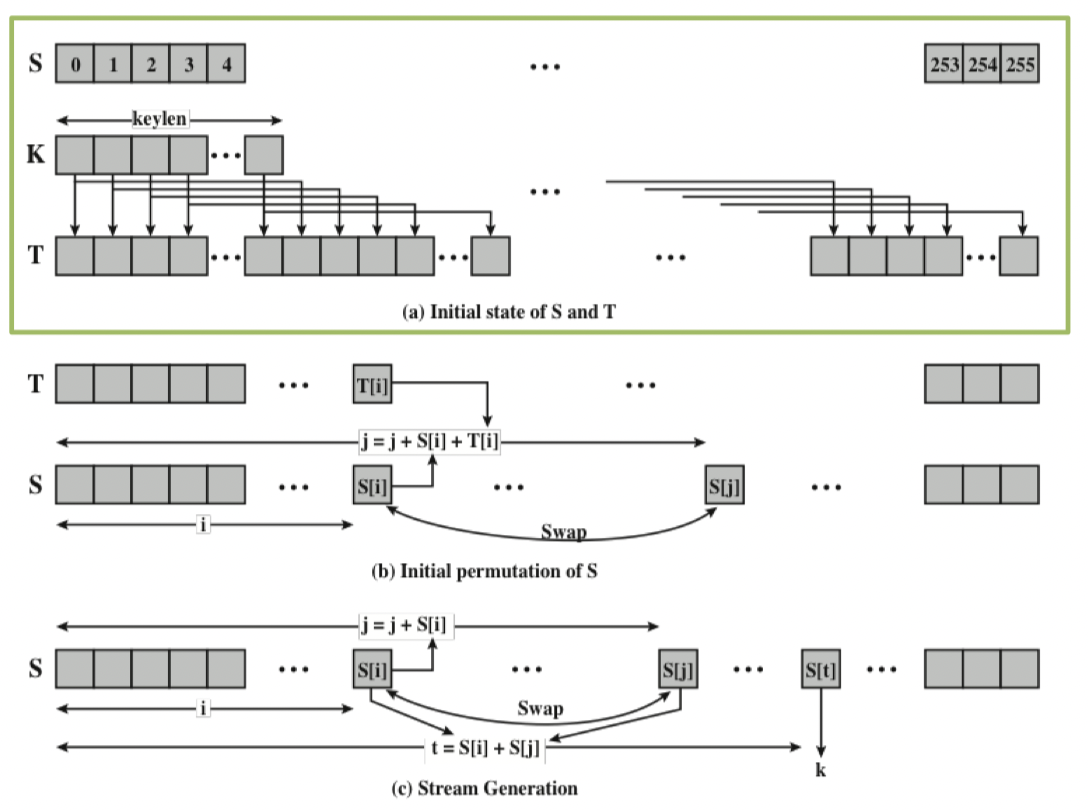
\includegraphics[scale=0.7]{images/rc4.png}}
\end{center}

\section{Public Key Crypto}
Public-key cryptography (or asymmetric cryptography) is a cryptographic system that uses pairs of keys. Each pair consists of a \textit{public key}, which may be known to others, and a \textit{private key}, which may not be known by anyone except the owner. The generation of such key pairs depends on cryptographic algorithms which are based on mathematical problems termed \textit{one-way functions}.

\subsection{Diffie-Hellman-Merkle (DHM) Key Exchange}
In order to understand how DHM works, we need to introduce some concepts.
\paragraph{Primitive root} A number $a$ is a \textit{primitive root} of prime number $p$ if the numbers $a\Mod{p},a^2\Mod{p},...,a^{p-1}\Mod{p}$ generate all the integers from $1$ to $p-1$ in some permutation (not all integers have primitive roots)

\paragraph{Discrete Logarithm} For any integer $b$ and primitive root $a$ of prime $p$ we can find a unique exponent $i$ s.t. $b\equiv a^i \Mod{p}$, with $i\in[0,p-1]$

\subsubsection{DHM steps}
In order to obtain a shared secret, Alice and Bob perform the following steps
\begin{enumerate}
    \item They publicly agree on $g$ (base) and $p$ (prime), where $g$ is primitive root of $p$.
    \item They both pick a secrete value, respectively $A$ and $B$
    \item They send each other respectively $g^A\Mod{p}$ and $g^B\Mod{p}$
    \item They both raise the received message to the power of their private key, computing the same value $g^{AB}\Mod{p}$, that is now their shared secret
\end{enumerate}
The only public information that an attacker has are $(g,p)$, so he needs to find $(A,B)$ to compute the secret, but this is an hard problem to solve (\textit{discrete logarithm problem}). $g$ has to be a primitive root of $p$, in order to maximize the keyspace.
\subsubsection{Man-in-the-Middle Attack}
After Alice and Bob choose publicly $(g,p)$ and privately $(A,B)$, Mallory (an attacker) could do the following
\begin{enumerate}
    \item When Alice and Bob try to communicate, Mallory can intercept their message and answer to them with $g^M\Mod{p}$ (where $M$ is a private value of Mallory)
    \item Both Alice and Bob end up computing a shared secret with Mallory, respectively $g^{AM}\Mod{p}$ and $g^{BM}\Mod{p}$, and Mallory does the same
    \item Alice and Bob think that they are now sharing a secret, but they are actually communicating with Mallory, that can read every message and send it to the actual receiver
\end{enumerate}

\subsection{RSA}
While DHM provides only encryption, RSA allow both encryption and authentication:
\begin{itemize}
    \item if Alice wants to encrypt a message $m$ to make it decryptable only for Bob, she can just encrypt it with Bob's public key
    \item if Alice wants to send a message $m$ adding her digital signature, she can just encrypt it with her private key
\end{itemize}
\subsubsection{Mathematical background}
In order to understand how RSA works, we need to learn some concepts


\paragraph{Totient} the totient $\phi(n)$ of a number $n$ is the amount of number coprime with $n$. If $n=pq$ with $(p,q)$ primes, we know that $\phi(n)=(p-1)(q-1)$


\paragraph{Euler's Theorem} In general \begin{itemize}
    \item $a^b\Mod{n}=a^{(b\mod{\phi(n))}}\Mod{n}$
    \item $b=1\Mod{\phi(n)} \implies a^b\Mod{n}=a$
\end{itemize}


\paragraph{}



\subsubsection{RSA steps}
\begin{enumerate}
    \item Choose two large primes $(p,q)$
    \item Compute $n=pq$
    \item Choose $e$ s.t. $\texttt{gcd}(e,\phi(n))$
    \item Find the multiplicative inverse $d$ s.t. $d\cdot e=1\Mod{\phi(n)}$
    {\color{teal} \item Public key $E=[e,n]$, private key $D=[p,q,d]$}
    \begin{itemize}
        \item \textbf{Encrypt}: $c=m^e\Mod{n}$
        \item \textbf{Decrypt}: $m=c^d\Mod{n}$
        \item \textbf{Verify}: $m=s^e\Mod{n}$
        \item \textbf{Sign}: $s=m^d\Mod{n}$
    \end{itemize}
\end{enumerate}

\subsubsection{PowerMod}
\textit{PowerMod} is a technique to easily compute large powers in modular arithmetic. Given a base $g$, an exponent $e$ and a modulo $p$, the steps to follow are the following:
\begin{enumerate}
    \item Convert $e$ to base 2
    \item Initialize $x=g$, start from the leftmost bit of $e$ (skip the first $1$)
    \begin{itemize}
        \item if the current bit is $0$, $x=x^2\Mod{p}$
        \item if the current bit is $1$, $x=(x^2\Mod{p})\cdot g \Mod{p}$
    \end{itemize}
\end{enumerate}

\subsubsection{Extended Euclidean Algorithm}
We use this algorithm to solve the problem of finding the  multiplicative inverse. Its goal is to find $(x,y)$ s.t.
\begin{equation*}
    ax+by=k=\texttt{gcd}(a,b)
\end{equation*}
This helps us in finding the multiplicative inverse because, if $\texttt{gcd}(a,b)=1$, we have that $ax+by=1$. If we set $a=\phi(n)(=\phi)$ and $b=e$, we can say
\begin{align*}
    [\cancel{(\phi x \Mod\phi)} + (ey \Mod\phi)]\Mod\phi\equiv 1 \Mod\phi \\
    ey\equiv 1 \Mod\phi
\end{align*}
This confirms that $\texttt{gcd}(e,\phi)=1$ and finds $d=y$

\paragraph{Steps}
\begin{wraptable}{r}{0.3\textwidth}
\vspace{-10pt}
\begin{tabular}{|c| c| c| c| c|} 
\hline
i & r_i & q_i & x_i & Y_i \\ [0.5ex] 
\hline\hline
-1 & 1759 &  & 1 & 0\\ 
0 & 550 &  & 0 & 1\\
1 & 109 & 3 & 1 & -3\\
2 & 5 & 5 & -5 & 16\\
3 & 4 & 21 & 106 & -339\\
4 & 1 & 1 & -111 & {\color{blue} \textbf{355}}\\
5 & 0 & 4 & & \\
\hline
\end{tabular}
\end{wraptable}


\begin{itemize}
    \item Initialization
    \begin{itemize}
        \item $r_{-1}=a \hspace{2em}-r_0=b$
        \item $x_{-1}=1 \hspace{2em}-x_0=0$
        \item $y_{-1}=0 \hspace{2em}-y_0=1$
    \end{itemize}
    \item Each step, compute
    \begin{itemize}
        \item $r_{i+1}=r_{i-1} \Mod{r_i}$
        \item $-q_{i+1}=\lfloor r_{i-1}/r_i\rfloor$
        \item $x_{i+1}= x_{i-1}-q_{i+1}x_i$
        \item $-y_{i+1}=y_{i-1}-q_{i+1}y_i$
    \end{itemize}
    \item Stop and find $d=y_n$ when $r_{n+1}=0$
\end{itemize}
Assume we are looking for multiplicative inverse of $e=550 \Mod{p=1759}$. See the result on the table.
\section{Hashes}
As we have seen in the previous chapters, if we want to guarantee both confidentiality and authentication with public crypto, the sender needs to encrypt the message with his private key (authenticity) and with the receiver public key (confidentiality). To reduce the computational burden we can use hash functions.\\
A hash function is a function that maps an arbitrary length input into a finite length output of $2^n$ bits (called \textit{message digest} or \textit{hash}).
If Alice wants to send a message to Bob, we can exploit hash functions in the following way:
\begin{wrapfigure}{r}{0.3\textwidth}
\vspace{50pt}
\fbox{
\includegraphics[scale=0.40]{images/hash.png}}
\end{wrapfigure}
\begin{enumerate}
    \item Alice computes the hash $h$ of the message $m$, encrypts it with her private key, and creates the new message $m'=m||E(D_A,h)$
    \item Alice encrypts $m'$ with the public key of Bob, generating $c=E(E_B,m')$
    \item Bob receives $c$, decrypts it with his private key, obtaining $m'$
    \item Bob separates $m$ from $E(D_A,h)$ and decrypts the latter with Alice's public key, obtaining $h$
    \item Bob verify the authenticity of the message simply computing the hash of the message $m$ and comparing it with $h$
\end{enumerate}
%\begin{center}
%    \includegraphics[scale=0.7]{hash.png}
%\end{center}

\subsection{Hash functions requirements}
A good hash function has by definition the following property:
\begin{itemize}
    \item \textbf{One-Wayness}: For any given image $h$ it is computationally infeasible to find pre-image $x$ s.t. $H(x) = h$
    \item \textbf{Weak collision resistance}: For any given pre-image $x$ it is computationally infeasible to find a pre-image $y\neq x$ with $H(x)=H(y)$
    \item \textbf{Strong collision resistance}: it is computationally infeasible to find any pair of pre-images $(x,y)$ s.t. $H(x)=H(y)$
\end{itemize}
\subsection{Birthday Attack}
It is clear that we need weak collision resistance property to obtain authenticity, but why do we need the strong collision resistance? The reason is that, without this property, it is possible to perform a birthday attack. A birthday attack is a type of cryptographic attack that exploits the mathematics behind the \textit{birthday problem}.
\subsubsection{Birthday Problem}
The birthday problem asks for the probability that, in a set of $n$ randomly chosen people, at least two will share a birthday. The birthday paradox is that, counterintuitively, the probability of a shared birthday exceeds 50\% in a group of only $23$ people. This can be proved using statistics:
\begin{itemize}
    \item Given $n$ people and $k$ days in a year, we have a probability\\ $P=1-\frac{(k-1)!}{k^{n-1}(k-n)!}$ that two of them share the birthday
    \item with $n=23$ and $k=365$, $P=1-\frac{364!}{365^{22}(365-23)!}\approx1-0.49=0.51$
\end{itemize}
\subsubsection{Applications}
We can exploit the birthday problem in the following way:
\begin{itemize}
    \item Prepare $2^{m/2}$ variations of valid and fraudulent messages each
    \item This should give us a $50\%$ chance of finding collision between a valid and a fraudulent message
    \item Now we can get someone to sign hash the valid message and then replace it with the fraudulent one
\end{itemize}

\newpage
\subsection{Hash Algorithms}
A generic hash algorithm works in the following way:
\begin{center}
    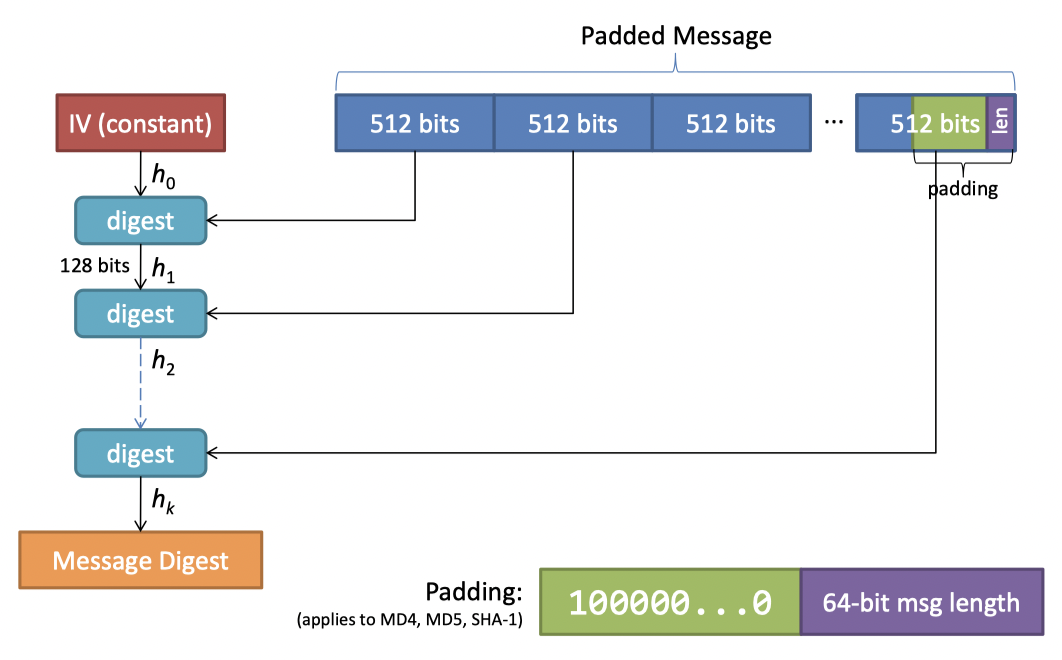
\includegraphics[scale=0.6]{hashfunc.png}
\end{center}

\subsubsection{MD5}
\begin{center}
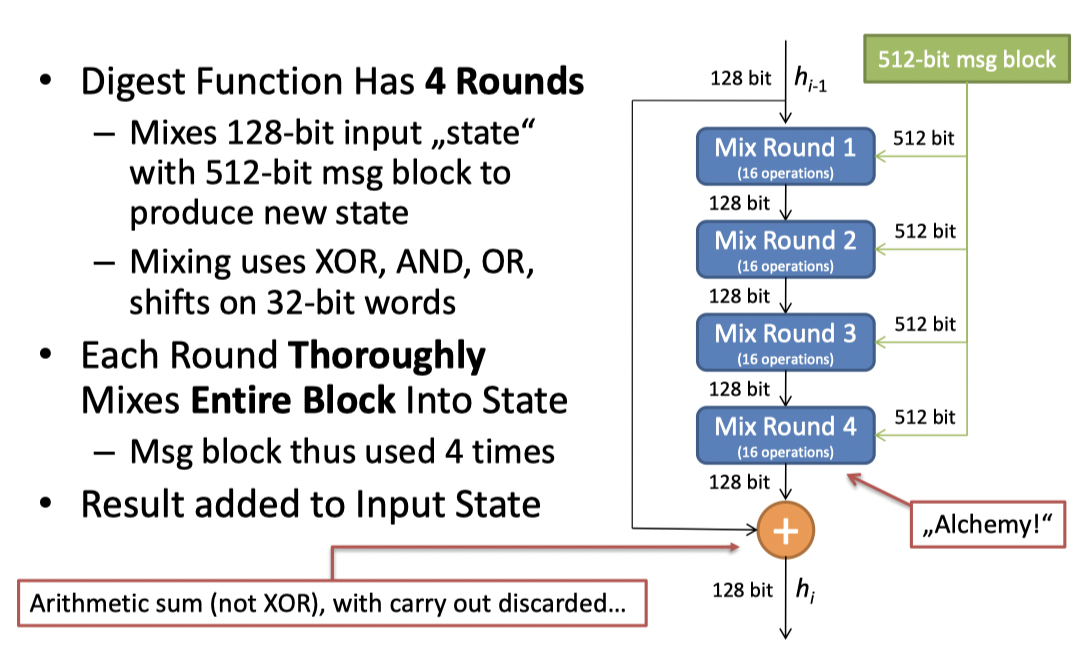
\includegraphics[scale=0.7]{md5.png}
    
\end{center}
\subsubsection{SHA1}
\begin{center}
    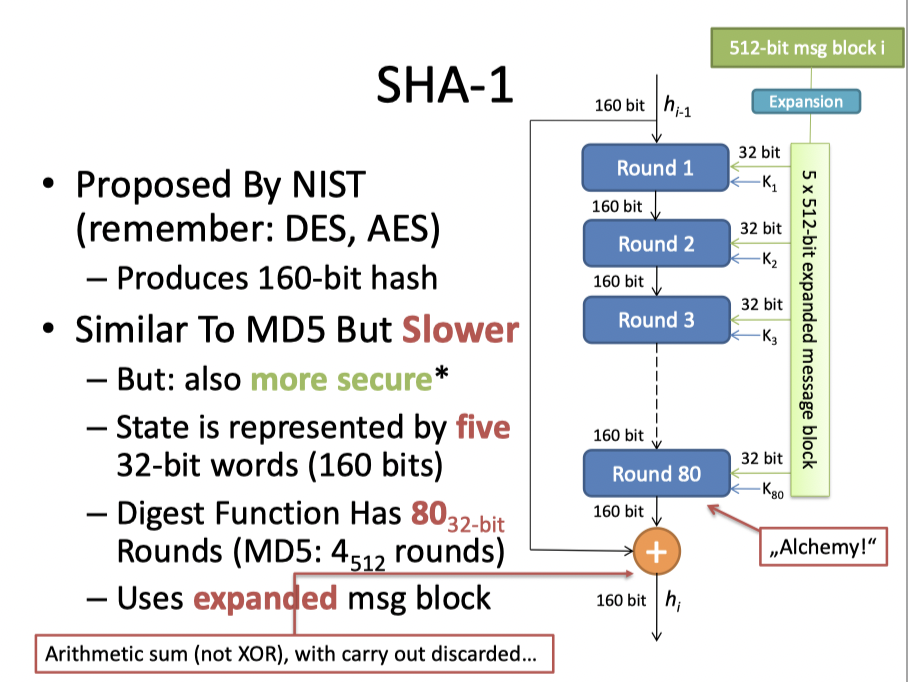
\includegraphics[scale=0.5]{sha1.png}    
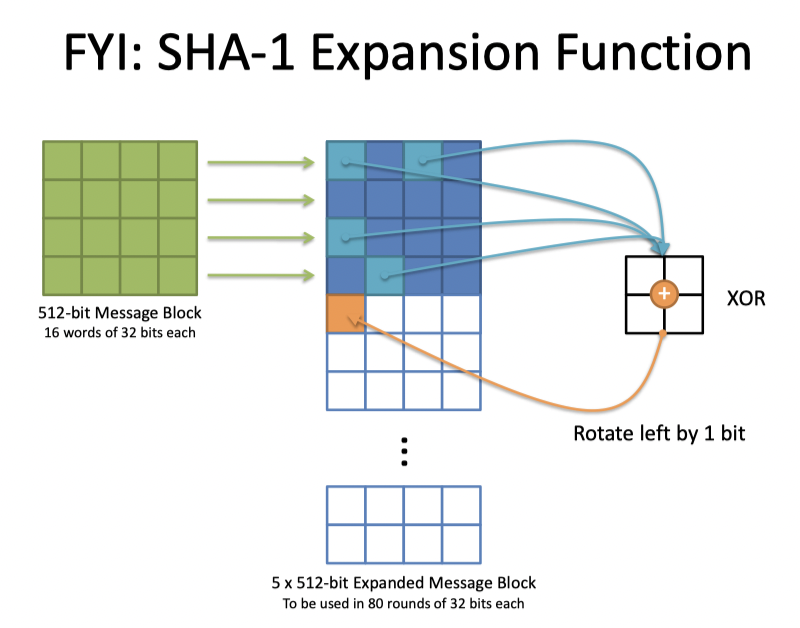
\includegraphics[scale=0.3]{sha1expfunc.png}
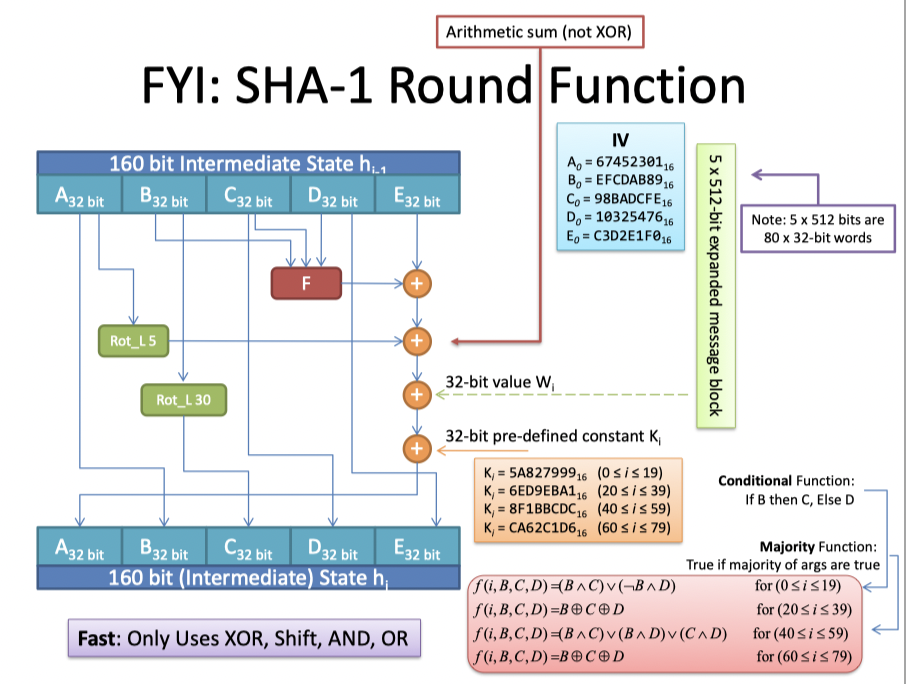
\includegraphics[scale=0.5]{sha1round.png}
\end{center}



\section{Macs}
A Message Authentication Code (MAC) is a short piece of information used for authenticating a message. It uses a shared secret key to provide integrity and authenticity, but differently from symmetric encryption it is not reversible. To do so, we can use hash functions or symmetric block cipher.\\
We can use hashes as MAC, but we have to be cautious on constructing them: if we use MAC$=MD(K_{AB}||msg)$, someone could perform a \textit{length extension attack}:
\begin{itemize}
    \item Alice sends "message, MAC" to Bob
    \item an attacker can construct an extension MAC'$=MD(MAC||msg')=MD(K_{AB}||msg||msg')$
\end{itemize}
To avoid this, we can construct the MAC differently:
\begin{itemize}
    \item MAC$=MD(msg||K_{AB})$
    \item Use only half of $MD$ (not extensible)
    \item Use MAC$=MD(MD(K_{AB}||msg))$
\end{itemize}

\subsection{HMAC}
HMAC is the standard MAC used in IPSec. It can use different hash functions, and what it does is to compute $h(K_{AB}\xor a || h(K_{AB}\xor b ||m))$, where $a$ and $b$ are two constants. With this structure, even if the attacker found $m'$ such that $m\neq m'$ and $h(m)=h(m')$, he would still be unable to "swap out" $m$ due to the prefixed key and the double hash.

\subsection{CBC-MAC}
An alternative to HMAC is CBC-MAC, that is simply the last ciphertext block of CBC (with $IV=0$). CBC-MAC is only secure for fixed length messages, because with variable-length messages with the same key $k$, an attacker who knows the MACs of two different messages $m_1$ and $m_2$ can easily compute the MAC of a third message $m_3$, even if he does not know the key $k$.
\begin{itemize}
    \item Assume the attacker know two messages and their MACs $(m_1,t_1)$ and $(m_2,t_2)$
    \item They create $m_3=m_1||m_2^*$, where $m_2^*$ is simply $m_2$ with the first block XORed with $t_1$
    \item They know the MAC of $m_3$ must be $t_2$
\end{itemize}

\subsection{Digital signatures vs. MAC}
We have to remember that there is a clear difference between digital signatures and MACs: a digital signature provides \textit{non-repudiation}, while MAC provides \textit{authenticity}

\section{Security Protocols}
Now that we have all the security primitives tools, we have to establish how should we use and combine them in order to have security protocols. We will examine three main type of protocols: authentication protocols, key distribution protocols and key establishment protocols.

\subsection{How to store sensible data}
Let's examine different login procedures, starting from naive approaches, understanding their problems and building up more safe ones.

\subsubsection{Password list} A list containing all user password is stored, and if a user try to login with password $pwd$, we search for $pwd$.

\subsubsection{Hashed password list} A list of hashed password is stored, if a user try to login with password $pwd$, we compute $hash(pwd)$ and search for it.
\paragraph{Attack 1} Pre-compute a lookup table of hashes for the most common passwords. It grows very large and very quickly
\paragraph{Attack 2} Use a \textbf{Rainbow table}:
\begin{enumerate}
    \item Find hashed password
    \item Use reduction function to convert to (pass-)word
    \item Try to find that word as an \textit{hash-chain end} in the table
    \begin{enumerate}
        \item If found, start from beginning of that hash-chain entry and hash/reduce/hash/reduce/etc, until you find password that hashes to observed hash
        \item If not found, hash the word and reduce it, then restart at step 2
    \end{enumerate}
\end{enumerate}
(N.B. a reduction function does not simply hash inverse, but map back the hash to the original password space $W$. Usually a rainbow table use different reduction function for each step)

\subsubsection{Salted hash} For each password choose a \textit{salt}, that is a random number, and save the salt alongside $hash(salt||pwd)$. Salt increases rainbow-table effort: for each bit of salt we need to double the number of rainbow tables, so with a large salt (e.g. 128 bit) it becomes unfeasible. 
\paragraph{Attack} Nonetheless, if the attacker gets access to the database the rainbow attacks becomes feasible (he would know the salt, that is saved in clear)

\subsubsection{Salted hash + pepper} To avoid the aforementioned problem, we can improve security using $pepper$, another random number that is stored separately from the password database and that is common for all the users. 
\paragraph{Attack} However, if even only one ($\texttt{salt + cleartext pwd})$ is known, the attacker could try to brute-force the pepper, so it must withstand brute-force attack (e.g. 112 bits)

\subsection{Authentication protocols}
In this section we will analyze how two entities can authenticates each other, avoiding attacks from malicious entities. We will focus on a family of protocols called \textit{Challenge-Response}, in which two nodes sends each other a value $N$ (the challenge) and expect some answer $f(K,N)$ (the response) from the other. As before, we will see different approaches, from the more naive to the more effective ones, keeping in mind that a good protocols should abide by the \textbf{Abadi-Needham} Protocols Design Guidelines:
\begin{itemize}
    \item \textbf{Be explicit} - every message should say what it means and its interpretation should only depend on its content. It's important to know clearly how encryption is used and how the timeliness of messages is proved
    \item \textbf{State your assumptions} - the conditions for a message to be acted upon should be clearly set out so that someone reviewing a design may see whether they are acceptable or not
\end{itemize}

\subsubsection{Mutual Authentication}
\begin{enumerate}
    \item $A\rightarrow B:\hspace{1em} A||N_1$
    \item $B\rightarrow A:\hspace{1em} N_2||f(K_{AB},N_1)$
    \item $A\rightarrow B:\hspace{1em} f(K_{AB},N_2)$
\end{enumerate}
\paragraph{Reflection Attack} If the attacker $T$ start this protocol twice, he can authenticate in the following way:
\begin{enumerate}
    \item $T\rightarrow B:\hspace{1em} A||N_1$
    \item $B\rightarrow T:\hspace{1em} N_2||f(K_{AB},N_1)$
    {\color{teal} \item{$T\rightarrow B:\hspace{1em} A||N_2$}}
    {\color{teal} \item $B\rightarrow T:\hspace{1em} N_3||f(K_{AB},N_2)$}
    {\color{teal} \item $\texttt{[close]}$}
    
    \item $T\rightarrow B:\hspace{1em} f(K_{AB},N_2)$
\end{enumerate}

\subsubsection{Mutual Authentication with Trusted Server}
Let's suppose that we have a trusted Key Distribution Center, or KDC (we will talk about them later), so that each node needs only one key shared with KDC. 

\subsubsection{Woo\&Lam}
\begin{enumerate}
    \item $A\rightarrow B:\hspace{1em} A$
    \item $B\rightarrow A:\hspace{1em} N_B$
    \item $A\rightarrow B:\hspace{1em} E(K_{AS},N_B)$
    \item $B\rightarrow S:\hspace{1em} E(K_{BS}, A||E(K_{AS},N_B))$
    \item $S\rightarrow B:\hspace{1em} E(K_{BS},N_B)$
\end{enumerate}
This authentication does not follow the Abadi-Needham rules.
\subsubsection{Fixed Woo\&Lam}
\begin{enumerate}
    \item $A\rightarrow B:\hspace{1em} A$
    \item $B\rightarrow A:\hspace{1em} N_B$
    \item $A\rightarrow B:\hspace{1em} E(K_{AS},N_B)$
    \item $B\rightarrow S:\hspace{1em} \textbf{A}||E(K_{AS},N_B)$
    \item $S\rightarrow B:\hspace{1em} E(K_{BS},\boldsymbol{A}||N_B)$
\end{enumerate}
Now the nonce $N_B$ is used only for freshness (and not for association), and there is no double encryption in step 4


\subsection{Key establishment protocols}
First of all, we want to introduce the concept of session key. A \textbf{session key} is a single-use symmetric key used for encrypting all messages in one communication session. There are different advantages on using session keys:
\begin{itemize}
    \item they limit the amount of ciphertext available
    \item different keys for authentication \& integrity protection
    \item compromise of long-term secret $\nRightarrow$ decryption of old messages
\end{itemize}
\paragraph{Forward Secrecy}
\begin{enumerate}
    \item $A\rightarrow B:\hspace{1em} \{N_A\}_{E_B}$
    \item $B\rightarrow A:\hspace{1em} \{N_B\}_{E_A}$
    \item Session key is $K_S=N_A\xor N_B$
\end{enumerate}
\paragraph{Perfect Forward Secrecy} (use signed DHM)
\begin{enumerate}
    \item $\texttt{Alice}\rightarrow \texttt{Bob}:\hspace{1em} \{g||p||A\}_{D_A}\hspace{3em} (A=g^a\Mod{p})$
    \item $\texttt{Bob}\rightarrow \texttt{Alice}:\hspace{1em} \{B\}_{D_B}\hspace{3em} (B=g^b\Mod{p})$
    \item $K_S=g^{ab}\Mod{p}$
\end{enumerate}
\subsection{Key distribution protocols}
\subsubsection{Needham-Schroeder}
\begin{enumerate}
    \item $A\rightarrow S:\hspace{1em} A||B||N_1$
    \item $S\rightarrow A:\hspace{1em} E(K_{AS},[N_1,||B||K_{AB}||\underbrace{E(K_{BS},[K_{AB}||A])}_{\texttt{ticket}}])$
    \item $A\rightarrow B:\hspace{1em} E(K_{AB},N_2)||\texttt{ticket}$
    \item $B\rightarrow A:\hspace{1em} E(K_{AB},N_2-1||N_3)$
    \item $A\rightarrow B:\hspace{1em} E(K_{AB},N_3-1)$
\end{enumerate}
\paragraph{Attack} If we use ECB mode, an attacker can impersonate $A$. Moreover, the attacker could have cracked old session key $K_{AB}$.

\paragraph{Timestamp-based alternative}
\begin{enumerate}
    \item $A\rightarrow S:\hspace{1em} A||B$
    \item $S\rightarrow A:\hspace{1em} E(K_{AS},[\textbf{T}||B||K_{AB}||\underbrace{E(K_{BS},[K_{AB}||A||T])}_{\texttt{ticket}}])$
    \item $A\rightarrow B:\hspace{1em} E(K_{AB},N_1)||\texttt{ticket}$
    \item $B\rightarrow A:\hspace{1em} E(K_{AB},N_1-1||N_2)$
    \item $A\rightarrow B:\hspace{1em} E(K_{AB},N_2-1)$
\end{enumerate}
In this way, is harder for an attacker to reply to message $3.$ much later

\subsubsection{Kerberos Protocol}
Kerberos is an authentication protocol, that introduces two new entities:
\begin{itemize}
    \item \textbf{Authentication Server (AS)} - it provides authentication credentials aka \textit{ticket granting ticket} (TGT)
    \item \textbf{Ticket Granting Server (TGS)}: it provides the access to different services based on the TGT received
\end{itemize}
\paragraph{Overview}
\begin{enumerate}
    \item User logs on to workstation and requests service on host
    \item AS verifies user's access right in database, creates TGT and session key. Results are encrypted using key derived from user's password
    \item Workstation prompts user for password and uses password to decrypt incoming message, then sends ticket and authenticator that contains user's name, network address, and time to TGS
    \item TGS decrypts ticket and authenticator, verifies request, then creates ticket for requested server
    \item Workstation sends ticket and authenticator to server
    \item Server verifies that ticket and authenticator match, then grants access to service. If mutual authentication is required, server returns an authenticator
\end{enumerate}

{\color{red} Secure Protocol Design Principles?}
\section{Certificates}
There are several techniques that have been proposed for the distribution of public keys. Virtually all these proposals can be grouped into the four general schemes
\begin{itemize}
    \item \textbf{Public announcement}: low overhead, no infrastructure required, but no trust (anyone can announce anything)
    \item \textbf{Public Directory}: there is a trusted entity to manage central service, but it needs to be online all the time, it fails if records get compromised and the registration requires an identity check
    \item \textbf{Public Key Authority}: it automates key exchange process and provides freshness through timestamps, but has the same problems of public directory
    \item \textbf{Public Key Certificates}: distribution does not require central authority
\end{itemize}

\paragraph{Definition} A certificate is a digitally-signed statement that binds a public key to some identifying information. The signer of the certificate is called its \textit{issuer} and the entity talked about in the certificate is the \textit{subject} of the certificate.\\

\noindent In order to believe to a certificates, we need to trust the issuer/signer not to lie to use and we also need to believe that it is hard to forge the digital signature on a signed document
\subsection{Strategies for CA Hierarchies}
Generally,in order to obtain a certificate
\begin{itemize}
    \item A user has to ask a \textit{Certification Authority} (CA) that issues certificates and asks for one
    \item The CA verifies the claim the user is making
    \item CA then issues the user a certificate for his public key
\end{itemize}
There are different viable hierarchies model to do so
\subsubsection{Monopoly}
Choose a universally trusted organization, embed their public key in everything and give them universal monopoly to issue certificates, so that everyone get certificates from them. There are several problems with this model:
\begin{itemize}
    \item If no one else is allowed to create certs, there is no incentive to offer competitive prices
    \item Getting certificates for remote user will be insecure or expensive
    \item The security of the world depends on the honesty and competence of that one organization, forever
\end{itemize}
\paragraph{Variation} Adding \textit{Registration Authorities} (RAs) that are trusted by the CA, so everyone can ask certificates to RAs, who in turn will ask to CA. In this way we solve the distance problem, but not the other issues.
\subsubsection{Oligarchy}
Have multiple trusted CAs. 
\paragraph{Variation} Allow trusted CAs to issue certificates for other CAs to the list of trusted CAs. This is similar to the monopoly variation, but is less efficient (end user must verify multiple certificates), faster (less delay for RA to get certificate) and less secure (multiple CA means multiple keys to trust).

\subsubsection{Anarchy}
Anyone signs certificates for anyone else. It is similar to Oligarchy variation, but user must consciously configure starting certificates. The problems are that it is hard to scale (computationally difficult to find path), it is not practical to decide if certain path should be trusted (too many decisions for the end user).

\subsection{Certificate Format}
\begin{center}
    \fbox{
    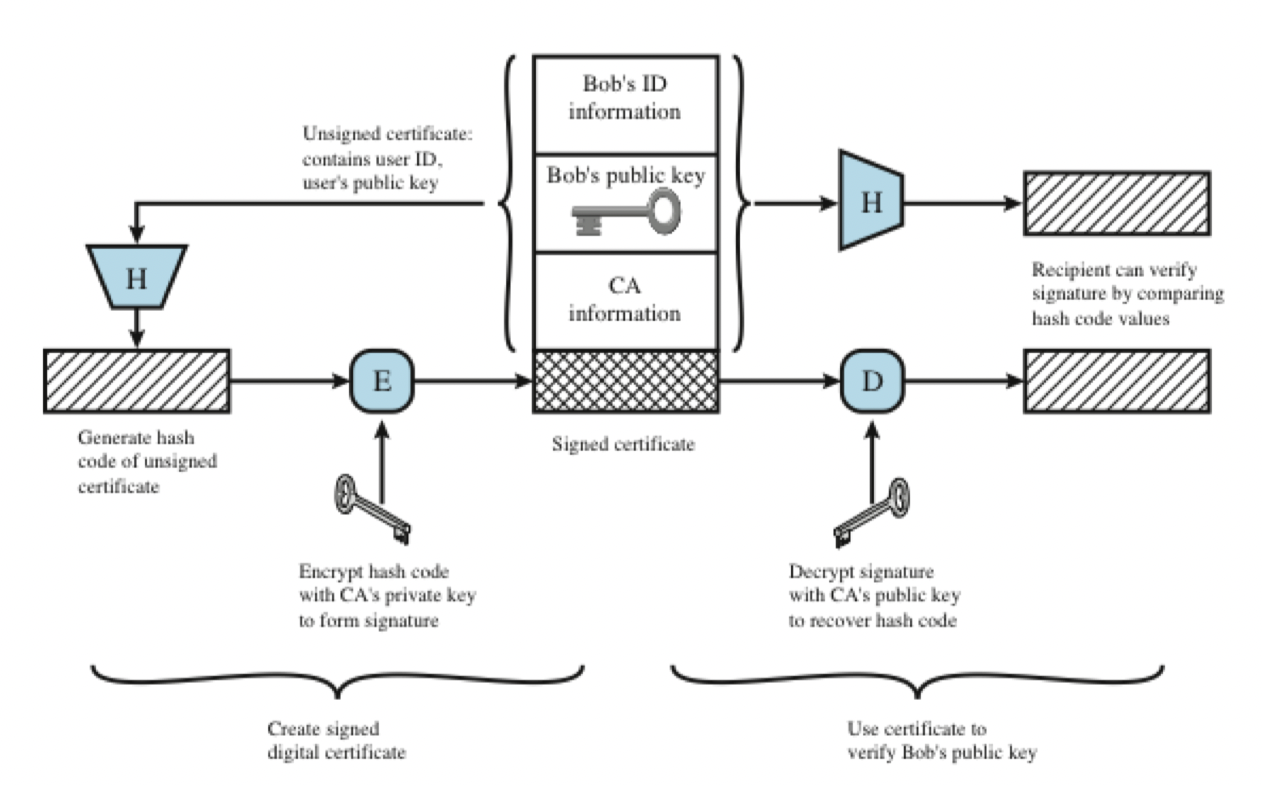
\includegraphics[scale=0.5]{images/certificate.png}}
\end{center}
The most common certificate format is \textbf{X.509}, containing a lot of information among which: serial number, issuer \& subject name, period of validity, signature.

\subsection{Certificate Lifecycle Management}
Lifecycle steps: enrollement, renewal \& revocation.
\subsubsection{Enrollement}
Enrollment is the process of obtaining a certificate from a CA.
\begin{enumerate}
    \item Alice generates a key pair, creates a message containing a copy of the public key and her identifying information, and signs the message with the private key (PKCS\#10).
    \begin{description}
    \item[Note:]Signing the message provided “proof-of-possession” (POP) of the private key as well as message integrity
    \end{description}
    \item CA verifies Alice’s signature on the message
    \item (Optional) CA verifies Alice’s ID through out-of-band means.
    \item CA creates a certificate containing the ID and public key, and signs it with the CA’s own key
    \begin{description}
    \item[Note:]CA has certified the binding between key and ID
    \end{description}
    \item Alice verifies the key, ID \& CA signature
    \item Alice and/or the CA publish the certificate
\end{enumerate}
\subsubsection{Revocation}
Each certificate includes a period of validity, but it may be desirable on occasion to revoke a certificate before it expires, for one of the following reasons:
\begin{itemize}
    \item The user’s private key is assumed to be compromised
    \item The user is no longer certified by this CA
    \item The CA’s certificate is assumed to be compromised
\end{itemize}
Each CA must maintain a \textit{Certification Revocation List} (CRL) consisting of all revoked but not expired certificates issued by that CA. Relying parties are expected to check CRLs before they rely on a certificate. Nevertheless, that are several problems with CRLs:
\begin{itemize}
    \item Not issued frequently enough to be effective against a serious attack
    \item Expensive to distribute (size \& bandwidth)
    \item Vulnerable to simple DOS attacks
    \item Can contain retroactive invalidity dates
    \item You can't revoke a CRL
\end{itemize}
For this reason, we use the \textit{Online Certs Status Protocol} (OCSP), that is designed for real-time responses to queries about the status of a single certificate (like a "selective" CRL).
\section{TLS}
\textit{Transport Layer Security} (TLS), the successor of the now-deprecated \textit{Secure Sockets Layer} (SSL), is a cryptographic protocol designed to provide communications security over a computer network. Here is how it works:
\begin{enumerate}
    \item $A\rightarrow B$: \textit{I want to talk} ($m_1$, aka “client\_hello”)
    \item $B\rightarrow A$: Certificate ($m_2$, aka “server\_hello”)
    \item $A\rightarrow B$: ($m_3$ , aka “client key exchange” \& “finished”)
    \item $B\rightarrow A$: ($m_4$, “finished”)
\end{enumerate}
TLS is composed by two layers of protocols:
\begin{enumerate}
    \item Record Protocol
    \item Handshake, Change Cipher Spec, Alert, Heartbeat Protocols
\end{enumerate}
In order to understand how TLS operates, we need to learn two architecture concepts:
\begin{itemize}
    \item \textbf{TLS connection}: connections are transient, every connection is associated with one session (one session can have multiple connections). The connection state parameters are: server and client random, server write key, client write key, server write MAC secret, client write MAC secret, IV (CBC mode), sequence numbers.
    \item \textbf{TLS session}: an association between a client and a server, created by the Handshake Protocol. Define a set of cryptographic security parameters which can be shared among multiple connections (used to avoid the expensive negotiation of new security parameters for each connection).
    The session state parameters are: session identifier, peer certificate, compression method, cipher spec, master secret, is\_resumable
\end{itemize}
\subsection{Record Protocol}
The TLS Record Protocol provides two services for TLS connections
\begin{itemize}
    \item Confidentiality: the Handshake Protocol defines a shared secret key that is used for conventional encryption of TLS payloads
    \item Message integrity: the Handshake Protocol also defines a shared secret key that is used to form a message authentication code (MAC)
\end{itemize}
Client and server each maintain a set of keys for sending and receiving (plus potentially an IV)
\subsection{Heartbeat Protocol}
The Heartbeat Protocol is a periodic signal generated by hardware or software to indicate normal operation or to synchronize other parts of a system (typically used to monitor the availability of a protocol entity). It consists of two message types, \texttt{hb\_request} and \texttt{hb\_response}. The heartbeat serves two purposes
\begin{itemize}
    \item It assures the sender that the recipient is still alive
    \item The heartbeat generates activity across the connection during idle periods, which avoids closure by a firewall that does not tolerate idle connections
\end{itemize}
\subsection{HTTPS}
HTTPS refers to the combination of HTTP and SSL to implement secure communication between Web browser and server. When HTTPS is used, the following elements of the communication are encrypted:
\begin{itemize}
    \item URL of the requested document
    \item Contents of the document
    \item Contents of browser forms
    \item Cookies sent
    \item Contents of HTTP header
\end{itemize}
\section{Computer Security}
Access Control (AC) is the set of (limited) action a user can do in a system. We use AC to prevent security breaches. The main access rights to data and programs are \texttt{read}, \texttt{write} and \texttt{execute}.
\subsection{General AC Principles}
\begin{itemize}
    \item System must first authenticate a user seeking access
    \item Then, AC reference monitor determines if specific requested access by this user is permitted
    \item A security administrator maintains an authorization database
    \item An auditing function monitors and keeps a record of user accesses to system resources (accountability, flaws)
\end{itemize}
\subsection{ACLs vs. Capabilities}
The authorization database can be organized in different way:
\begin{itemize}
    \item Access Control List (ACL), often used in filesystems, contains a list for each \texttt{object} containing the right of each \texttt{subject} on it
    \item Capabilities is the dual of ACL. It contains a list for each \texttt{subject} containing the right on each \texttt{object}
\end{itemize}
\subsection{UNIX Permissions}
UNIX used ACLs and for each \texttt{object}, it indicated the rights of the \textit{owner}, the \textit{group owner} and the \textit{world}
\paragraph{SUID}
UNIX also offer the possibility for using \textbf{SUID} root, that allow users to run an executable with the filesystem permissions of the executable's owner or group owner. They are often used to allow users on a computer system to run programs with temporarily elevated privileges in order to perform a specific task. The introduction of SUID root led to several security vulnerability.
\paragraph{\texttt{sudo}} A better solution could be to use \texttt{sudo}, allowing selected users to temporarily become root (authenticating with their \texttt{pwd})

\subsection{Types of AC Policies}
\begin{itemize}
    \item \textbf{Discretionary AC}: security decisions up to object owner, different defaults option possible, no coherent security policy enforceable
    \item \textbf{Mandatory AC}: system-wide security policy enforcement, all objects and subjects have "security labels", access granted iff security labels "match", allows control of information flows
\end{itemize}


\subsubsection{Mandatory Access Policies Policy}
\paragraph{BLP Model}
The Bell-La Padula Model consists of two properties:
\begin{itemize}
    \item \textbf{Read Down}: a \texttt{subject}'s must dominate the security level of the \texttt{object} being read. More formally, $S$ can read $O$ iff $L_S \geq L_O \cap C_S \supseteq C_O$ and $S$ has discretionary read access to $O$
    \item \textbf{Write Up}: a \texttt{subject}'s clearance must be dominated by the security level of the \texttt{object} being written to. More formally, $S$ can write to $O$ iff $L_S \leq L_O \cap C_S \subseteq C_O$ and $S$ has discretionary write access to $O$
\end{itemize}

\paragraph{Problem} High clearance subjects can never communicate with low clearance subjects, so we need dynamic security levels. BLP protects confidentiality, but not integrity

\paragraph{Biba Model}
It is a state machine model to ensure integrity with these property:
\begin{itemize}
    \item \textbf{No Read Down}: a \texttt{object}'s integrity level must dominate the integrity level of the \texttt{subject} reading it ($I_O \geq I_S$)
    \item \textbf{No Write Up}: a \texttt{subject}'s integrity level must dominate the integrity level of the \texttt{object} being written to ($I_S \geq I_O$)
\end{itemize}
\section{Web Security}
\subsection{HTTP Authentication}
\paragraph{Basic}
The browser sends password in the clear (over encrypted connection HTTPS). The server has \texttt{.htpasswd} file containing hashed passwords.
\paragraph{Digest}
Uses nonces, timestamps, MD5 hashes, "opaque" server data.\\\\
In practice, neither method is much used anymore, because they are not optimal for user experience (login process). The most used approach is to use HTTPS + HTML form.

\subsection{DNS Spoofing}
\textit{Domain Name Server} (DNS) spoofing is an attack in which altered DNS records are used to redirect online traffic to a fraudulent website that resembles its intended destination. The strategy used is the following:
\begin{enumerate}
    \item User wants to connect to \texttt{www.site.com}
    \item Local DNS resolver sends UDP packet to DNS server for IP address
    \begin{description}
    \item[Note:] The first "matching" reply will be used to cache IP, so if attacker is faster than DNS resolver, his IP gets used
    \end{description}
    \item The attacker listen to outgoing traffic, identify DNS packets and send "fake" reply packets that match the query
\end{enumerate}
\textit{DNS-over-TLS} (DoT)/\textit{-over-HTTP} (DoH) adds confidentiality to DNS.

\subsection{Homograph Attacks}
Homograph attack is a way a malicious party may deceive computer users about what remote system they are communicating with, by exploiting the fact that many different characters look alike (e.g. latin letter vs. cyrillic letter). These type of attack are usually done to commit \textit{phishing} (obtain sensitive information by disguising as a trustworthy entity). A (partial) solution to this is \textit{Punycode}: in case a internet hostname contains letter of different alphabets, it get displayed in a easily detectable format (this solution does not hold if we use letters of only one alphabet).


\subsection{Man-in-the-Middle SSL Attack}
Due to a bug on Internet Explorer 7, leaf certificates can sign other leaf certificates, so an attacker can sign any SSL certificate, "proving" to a client that it is using the authentic site.


\subsection{XSS - Cross Site Scripting Attack}
Inject malicious script code into a (trusted) webpage a user is viewing, so that user‘s browser executes malicious code (the user will probably assume that the behavior is part of the original site). XSS is possible exploiting JavaScript issues, such as the fact that it can access and change any part of a web page. For this reason JavaScript added the \textit{Same Origin Policy} (SOP): origin needs to match domain, protocol \& port in order to read/write on the site.
Another powerful way to avoid XSS is NoScript, a browser extension that allow JavaScript on originating server only


\subsection{SQL Injection}
SQL injection is a code injection technique used to attack data-driven applications, in which malicious SQL statements are inserted into an entry field for execution (e.g. to dump the database contents to the attacker). SQL injection must exploit a security vulnerability in an application's software (e.g. user input is incorrectly filtered for string literal escape characters embedded in SQL statements).
\section{Software Security}
\subsection{The 7 Sins of Insecure Software}
\begin{enumerate}
    \item Improper input validation / representation
    \item API abuse
    \item Incorrect use/coding of security constructs
    \item Incorrect assumptions re. time / state
    \item Improper error handling According to
    \item Incorrect assumptions regarding execution environment
\end{enumerate}

\subsection{Common Input Validation Errors}
\begin{itemize}
    \item \textbf{Buffer Over-Read}: Reading beyond boundaries of allocated memory (disclose secret data in adjacent memory cells)
    \item \textbf{Buffer Overflow}: Writing outside boundaries of allocated memory (crash, corrupt data, execute malicious code)
    \item \textbf{String Termination Error}: Relying on proper string termination (buffer overflow)
    \item \textbf{Format String}: Allowing an attacker to control printf format string (buffer overflow)
    \item \textbf{Integer Overflow}: Not accounting for integer overflow (logic errors, buffer overflow)
    \item \textbf{Command Injection}: Executing commands from untrusted source (execute malicious commands)
    \item \textbf{SQL Injection}: Exec SQL statements using unvalidated user input (execute arbitrary SQL commands)
    \item \textbf{Cross-Site Scripting}: Sending unvalidated data to Web client (execute malicious commands on trusted site)
\end{itemize}

\subsection{Buffer Overflow}
Buffer overflow is an anomaly where a program, while writing data to a buffer, overruns the buffer's boundary and overwrites adjacent memory locations. By sending in data designed to cause a buffer overflow, it is possible to write into areas known to hold executable code and replace it with malicious code.\\
It is possible to fit arbitrary-sized shellcode on the stack: start shellcode after return address and fill the rest with “NOPsled”, in this way the return address needs to just point somewhere before shellcode.

\paragraph{Protecting the stack}
\begin{itemize}
    \item Make stack non-executable
    \item Use \textit{Canary} to detect overflows
    \item Use separate stack for return address
\end{itemize}
\paragraph{Heap Corruption} Occurs when a program damages the allocator's view of the heap.
\paragraph{Format String} Occurs when the submitted data of an input string is evaluated as a command by the application. In this way, the attacker could execute code, read the stack, or cause a segmentation fault in the running application, causing new behaviors that could compromise the security or the stability of the system.

\subsection{Incorrect use of Time/State}
\paragraph{TOCTTOU} \textit{Time-of-check to Time-of-use} is a class of software bugs caused by a race condition involving the checking of the state of a part of a system (such as a security credential) and the use of the results of that check.

\subsection{The Saltzer-Schroeder Security Principles}
\begin{enumerate}
    \item \textbf{Fail-Safe Defaults}: protection mechanism should deny access by default, and grant access only when explicit permission exists.
    \item \textbf{Complete Mediation}: mechanism should check every access to every object.
    \item \textbf{Least Privilege}: mechanism should force every process to operate with the minimum privileges needed to perform task.
    \item \textbf{Open Design}: protection should not depend on attackers being ignorant of its design to succeed. It may however be based on the attackers’ ignorance of specific information such as passwords or cipher keys.
    \item \textbf{Separation of Privilege}: protection mechanism should grant access based on more than one piece of information.
    \item \textbf{Economy of Mechanism}: the protection mechanism should have a simple and small design.
    \item \textbf{Least Common Mechanism}: the protection mechanism should be shared as little as possible among users (e.g., process isolation).
    \item \textbf{Psychological Acceptability}: the protection mechanism should be easy to use (at least as easy as not using it).
\end{enumerate}

\end{document}             % End of document.